\documentclass{beamer}

\usepackage{fancyvrb,tikz, dsfont}

\usetikzlibrary{automata,arrows}

\usetheme{Dresden}

\mode<presentation>

\title[Asteria]{Asteria}
\subtitle{A High Performance 3D Game Engine}
\author{Samuel Payson \and Akanksha Vyas}

\begin{document}

\begin{frame}
\titlepage
\end{frame}

\section{Introduction}

\subsection{Project Goals}

\begin{frame}
   \frametitle{Project Goals}
   \begin{enumerate}
      \item Build an open source game engine
      \item High performance
      \item Provide good documentation
      \begin{itemize}
         \item New developers should be able to join the project without first
         ``reverse engineering'' all past work
         \item One thing missing from most open source projects is
         documentation of high-level design
      \end{itemize}
   \end{enumerate}
\end{frame}

\begin{frame}
   \frametitle{Why Reinvent the Wheel?}
   \begin{itemize}
      \item Learning Experience
      \begin{itemize}
         \item Good way to understand the challenges of building a game
         \item Learn OpenGL and related technologies
      \end{itemize}
      \item Most existing open source engines are bloated
      \item Building things is fun!
   \end{itemize}
\end{frame}

\section{Semester Goals}

\subsection{What We Set Out to Do}

\begin{frame}
   \frametitle{What Did We Do This Semester?}
   \begin{enumerate}
      \item Solid design before implementation.
      \item Animation subsystem (Doom 3's \texttt{md5} file format)
      \item Resource Manager
      \item Abstract interface to OpenGL
   \end{enumerate}
\end{frame}

\subsection{Accomplishing Our Goals}

\begin{frame}
   \frametitle{Design Before Implementation}
   \begin{itemize}
      \item Decide how code will be structured before writing it
      \item Consulted literature on the topic
      \begin{itemize}
         \item \emph{Game Engine Architecture} by \emph{Jason Gregory}
      \end{itemize}
      \item Balanced extensibility and performance
      \item Strive for abstractions that aid performance
   \end{itemize}
\end{frame}

\begin{frame}
   \frametitle{The Animation Subsystem}
   \begin{itemize}
      \item Based on Doom 3's \texttt{md5} file format.
      \item Skeletal animation with vertex skinning.
      \begin{itemize}
         \item Animations are described by the motion of 'joints'
         \item Vertices can be affected by one or more joints.
         \item Vertex final position at each frame decided by a weighted
         average of all joints affecting it.
      \end{itemize}
      \item Implemented using shaders on the GPU, allowing animations to scale
      smoothly with framerate.
   \end{itemize}
\end{frame}

\begin{frame}
   \frametitle{Components of the Animation Subsystem}
   \begin{itemize}
      \item The parser
         \begin{itemize}
            \item Parses a file and creates a structure that contains a list of
            frames. Each frame is a description of joints.
         \end{itemize}
      \item The Interpolation
         \begin{itemize}
            \item Using the description of two frames, it calculates the
            description of a frame between them. 
            \item Interpolation functions: LERP, SLERP and NLERP
         \end{itemize}
      \item The Draw Function
         \begin{itemize}
            \item Calculates position and orientation of each joint w.r.t its
            parent
            \item Sends each joint to the GPU
         \end{itemize}
   \end{itemize}
\end{frame}

\begin{frame}
   \frametitle{Resource Manager}
   \begin{itemize}
      \item \emph{Resources} are any kind of data that the game needs access to
      \begin{itemize}
         \item 3D Models
         \item Audio Files
         \item Images
      \end{itemize}
      \item Storing these as individual files on the disk requires expensive
      filesystem navigation every time a file must be loaded
      \item The \emph{Resource Manager} provides an efficient abstraction for
      these files
   \end{itemize}
\end{frame}

\begin{frame}
   \frametitle{The Resource Manager Illustrated}
   \begin{itemize}
      \item The code thinks it is dealing with real files, but in fact the Resource
      Manager is decompressing data from an archive on the fly
   \end{itemize}
   \begin{center}
      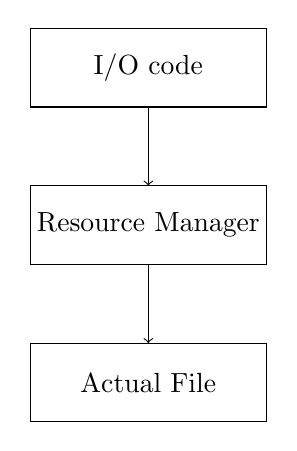
\begin{tikzpicture}
         \path[draw=black,->] (0,0) -- (0,-1);
         \path[draw=black,->] (0,-2) -- (0,-3);
         \path[draw=black] (-1.5,0) rectangle node {I/O code} (1.5,1);
         \path[draw=black] (-1.5,-2)   rectangle node {Resource Manager} (1.5,-1);
         \path[draw=black] (-1.5,-4)   rectangle node {Actual File} (1.5,-3);
      \end{tikzpicture}
   \end{center}
\end{frame}

\section{Conclusions}

\subsection{What We Learned}

\begin{frame}
   \frametitle{Design Lessons Learned}
   \begin{itemize}
      \item Had to swallow pride about Object Oriented Programming
      \begin{itemize}
         \item Switched from C to C++ halfway through the semester
         \item Problem fit very well into OOP design ideas
      \end{itemize}
      \item Testing is very worthwhile
      \item Abstraction can be useful for \emph{improving} performance, if used
      correctly
   \end{itemize}
\end{frame}

\begin{frame}
   \frametitle{Math and Technology}
   \begin{itemize}
      \item Learned a lot about OpenGL
      \item Quaternion Mathematics
      \item A lot about game design
      \item Object Oriented design strategies that are performance friendly
   \end{itemize}
\end{frame}

\subsection{Plans for the Project}

\begin{frame}
   \frametitle{Where do we go now?}
   \begin{itemize}
      \item Scene Graphs and World Representation
      \item Textures and Materials
      \item User Interface
      \item Scripting
      \item Physics Engine
   \end{itemize}
\end{frame}

\end{document}
